\frame
{
\frametitle{Análisis Cuantitativo de Riesgos}
\begin{itemize}
	\item Este proceso usa \emph{técnicas y métodos} \textbf{estadísticos} para:
	\begin{itemize}
		\item Cuantificar los \emph{posibles resultados} del proyecto y sus probabilidades
		\item Evaluar la \emph{probabilidad de lograr} los \textbf{objetivos} específicos del proyecto.
		\item Identificar los riesgos que requieren una \textbf{mayor atención}.
	\end{itemize}
\end{itemize}
\begin{columns}
	\begin{column}{0.6\textwidth}
	\end{column}
	\begin{column}{0.4\textwidth}
		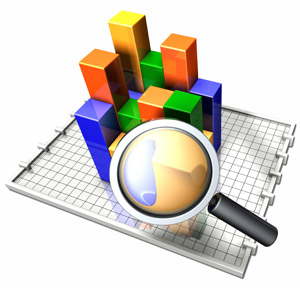
\includegraphics[width=3cm]{img/quantity}
	\end{column}
\end{columns}
}

\frame
{
\frametitle{Análisis Cuantitativo de Riesgos}
\begin{block}{Definición}
\begin{itemize}
	\item Analiza el efecto de esos riesgos y les asigna una \textbf{calificación numérica}.
	\item También presenta un método cuantitativo para \textbf{tomar decisiones} en caso de \emph{incertidumbre}. 
\end{itemize}
\end{block}
}


\frame
{
\frametitle{Análisis Cuantitativo de Riesgos}
\framesubtitle{Entradas}
\begin{columns}
	\begin{column}{0.8\textwidth}
		\begin{itemize}
			\item<1-> Registro de Riesgos.
			\item<2-> Plan de administración de \textbf{Riesgos}.
			\item<3-> Plan de administración de \textbf{Costos}.
			\item<4-> Plan de administración de \textbf{Planificación}.
			\item<5-> Activos organizacionales del Proceso.
		\end{itemize}
	\end{column}
	\begin{column}{0.2\textwidth}
		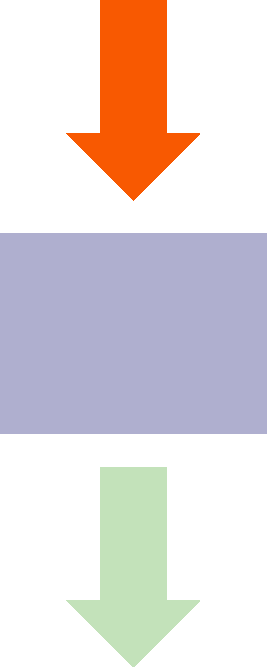
\includegraphics[width=2cm]{img/input}
	\end{column}
\end{columns}
}

\frame
{
\frametitle{Análisis Cuantitativo de Riesgos}
\framesubtitle{Herramientas y Técnicas}
\begin{columns}
	\begin{column}{0.8\textwidth}
		\begin{itemize}
			\item<1-> \emph{Recolección} de datos y técnicas de representación.
			\item<2-> Análisis cuantitativo de riesgos y técnicas de modelamiento.
			\begin{itemize}
				\item<3-> Análisis de sensibilidad.
				\item<4-> Análisis de valores de \emph{expectación monetaria}.
				\item<5-> Modelamiento  y simulación.
			\end{itemize}
			\item<6-> Juicio Experto.
		\end{itemize}
	\end{column}
	\begin{column}{0.2\textwidth}
		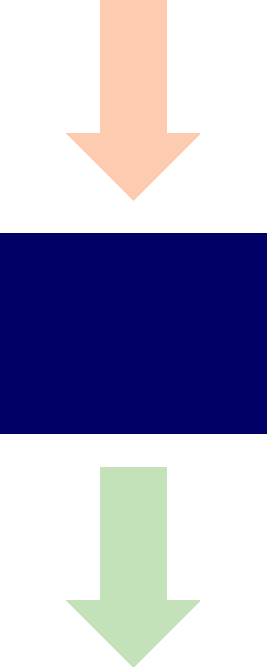
\includegraphics[width=2cm]{img/tools}
	\end{column}
\end{columns}
}

\frame
{
\frametitle{Análisis Cuantitativo de Riesgos}
\framesubtitle{Salidas}
\begin{columns}
	\begin{column}{0.8\textwidth}
		Actualización de los registros de riesgos.
		\begin{itemize}
			\item<1-> Análisis \textbf{probabilístico} del proyecto.
			\item<2-> Probabilidad de \emph{obtener} los objetivos de costo y tiempo.
			\item<3-> Lista \textbf{priorizada} de riesgos cuantificados.
			\item<4-> \textbf{Tendencias} en los resultados cuantitativos de análisis de riesgos.
		\end{itemize}
	\end{column}
	\begin{column}{0.2\textwidth}
		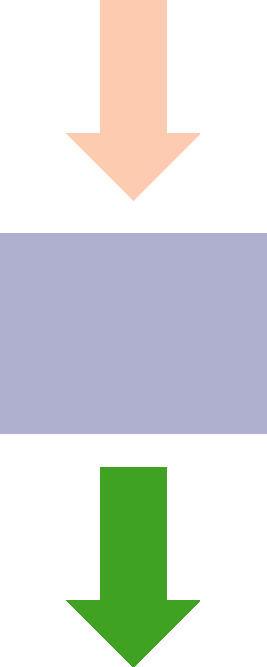
\includegraphics[width=2cm]{img/output}
	\end{column}
\end{columns}
}

